\documentclass[12pt, addpoints]{exam} % добавить или удалить answers в скобках, чтобы показать ответы
%\usepackage[T2A, T1]{fontenc}
%\usepackage[utf8x]{inputenc}
%\usepackage[greek, russian]{babel}
%\usepackage[OT1]{fontenc}


\usepackage{fontspec}
\usepackage{polyglossia}

\setdefaultlanguage{russian}
\setotherlanguages{english, greek}

\setmainfont[Ligatures=TeX]{Linux Libertine O}
% http://www.linuxlibertine.org/index.php?id=91&L=1

%\usepackage{mathtools}
\usepackage{comment}
\usepackage{booktabs}
\usepackage{amsmath}
\usepackage{tikz}
\usepackage{amsfonts}
\usepackage{amssymb}
\usepackage{icomma}
\usepackage[left=1cm,right=1cm,top=2cm,bottom=2cm]{geometry}
\DeclareMathOperator{\E}{\mathbb{E}}
\DeclareMathOperator{\Var}{\mathbb{V}\mathrm{ar}}
\DeclareMathOperator{\Cov}{\mathbb{C}\mathrm{ov}}
\DeclareMathOperator{\Corr}{\mathbb{C}\mathrm{orr}}
\DeclareMathOperator{\plim}{plim}
\let\P\relax
\DeclareMathOperator{\P}{\mathbb{P}}
\newcommand{\cN}{\mathcal{N}}
\newcommand{\hbeta}{\hat{\beta}}

\usepackage{floatrow}
%\newfloatcommand{capbtabbox}{table}[][\FBwidth]

\begin{document}

\pagestyle{headandfoot}
\runningheadrule
\firstpageheader{Теория вероятностей}{КосмоWAR, красные задачи}{17 декабря 2016}
\firstpageheadrule
\runningheader{Теория вероятностей}{КосмоWAR, красные задачи}{17 декабря 2016}
\firstpagefooter{}{}{}
\runningfooter{}{}{}
\runningfootrule

\hqword{Задача}
\hpgword{Страница}
\hpword{Максимум}
\hsword{Баллы}
\htword{Итого}
\pointname{\%}
%\renewcommand{\solutiontitle}{\noindent\textbf{Решение:}\par\noindent}
\renewcommand{\solutiontitle}{}

%Таблица с результатами заполняется проверяющим работу. Пожалуйста, не делайте в ней пометок.

%\begin{center}
%  \gradetable[h][questions]
%\end{center}

\vspace{0.2in}

\makebox[\textwidth]{Команда:\enspace\hrulefill}

\begin{center}
ЭРА I
\end{center}

\begin{questions}


\question Если последовательность случайных величин $\xi_n$ сходится к константе $c$ по распределению, то

$\lim\limits_{n\to\infty}\mathbb{P}(|\xi_n - c| \ge \varepsilon) = 0\,\,\forall \varepsilon > 0$.
\begin{solution}
Да.
\end{solution}

\question Вася проходит конкурс в школу космодесантников. Чтобы поступить в школу, необходимо пройти испытание лучше, чем 80$\%$ участников (а участников много, все хотят служить галактике!). Результаты испытаний имеют нормальное распределение с математическим ожиданием 500 и дисперсией 100. Вася набрал 512 баллов за испытание. Поступит ли Вася в школу?
\begin{solution}
да, поступит
\end{solution}



\question Пусть $X$ и $Y$~--- независимые случайные величины. Тогда $\mathbb{E}(XY) = \mathbb{E}(X)\mathbb{E}(Y)$. \begin{solution}
Да.
\end{solution}

\question В шестизарядный револьвер кладут два патрона подряд и раскручивают. Лермонтов делает выстрел, а после него выстрел обязан сделать Мартынов. Что выгоднее для Мартынова: раскрутить барабан или сразу сделать выстрел?
\begin{solution}
если пуля вылетела, то  лучше прокрутить барабан перед выстрелом; если пуля не вылетела, то  лучше сразу сделать выстрел.
\end{solution}

\question Пусть случайные величины $X$ и $Y$ независимы и обе распределены равномерно на отрезке $[0;1]$. Тогда $(X+Y)\sim U[0;2]$.
\begin{solution}
Нет.
\end{solution}


\question Некоррелированные нормально распределенные случайные величины независимы.
\begin{solution}
Нет.
\end{solution}

\question Пусть $X\sim \mathcal{N}(2; 5)$. Чему равно $\mathbb{E}(X^2)$?
\begin{solution}
9
\end{solution}

\question Случайная величина X принимает три значения 1, 2 и 3 с вероятностями 1/6, 2/6 и 3/6, соответственно. Найдите $P(X=3|X>1.5)$

\begin{solution}
$3/5$
\end{solution}

\question Лунтик подкидывает правильную игральную кость. С помощью неравенства Маркова оцените вероятность того, что у Лунтика выпадет число, не меньшее 5. Можно ли получить результат точнее (тогда чему равна эта вероятность)?
\begin{solution}
$\le 0,7$; $\dfrac{1}{3}$
\end{solution}

Если вы уже решили красные, а также синие и белые задачи, или если у вас ничего не получается решить, то можно раскрасить Лунтика, чтобы не скучать до конца тура!
\begin{center}
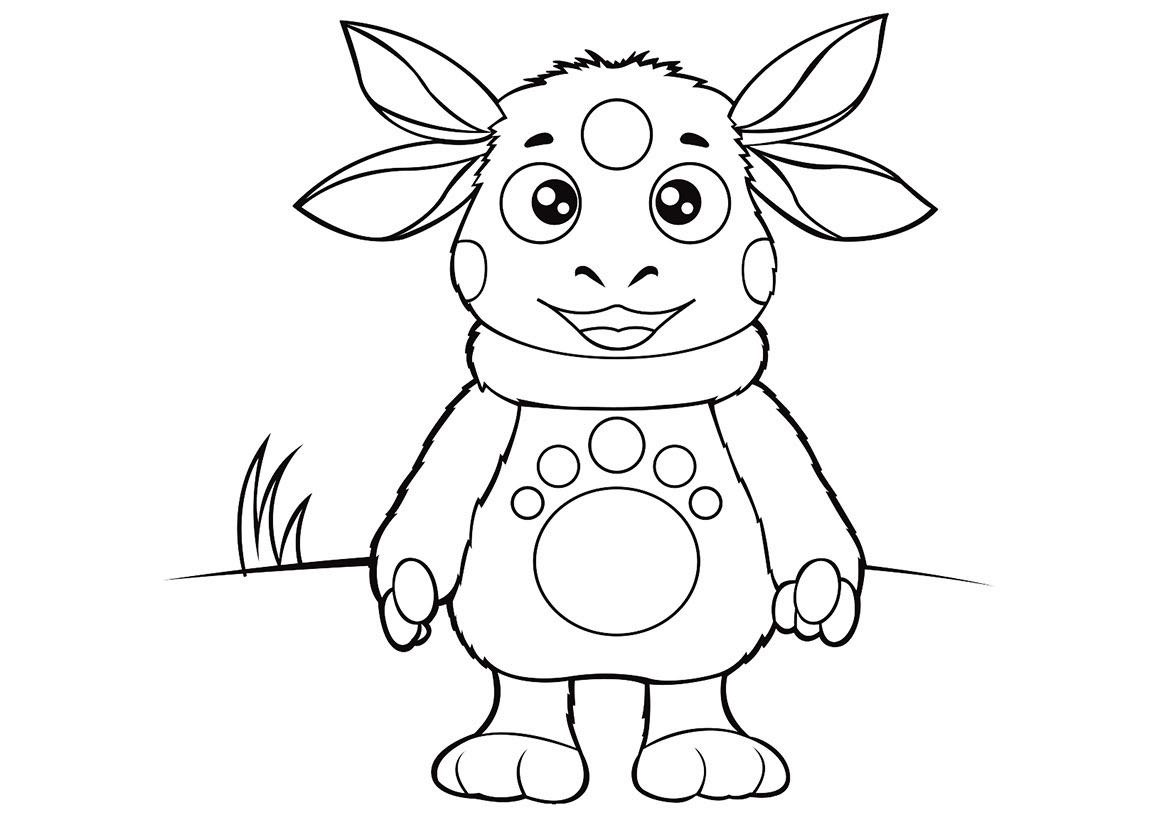
\includegraphics[scale=0.3]{luntik}
\end{center}

\end{questions}

\newpage
\vspace{0.2in}

\makebox[\textwidth]{Команда:\enspace\hrulefill}

\begin{center}
ЭРА II
\end{center}

\begin{questions}

\question Если $X\sim \mathcal{N}(0;1)$, $Y\sim \mathcal{N}(0;2)$ и $\Cov{(X, Y)} = 3$, то $X+Y\sim\mathcal{N}(0;3)$.
\begin{solution}
Нет.
\end{solution}

\question Британские ученые обнаружили в черной дыре две случайные величины: $X$ и $ Y=(X - E(X))^2$. С помощью неравенства Маркова оцените $P(Y \geq b^2)$. Что вам это напомнило?
\begin{solution}
$\dfrac{\Var{X}}{b^2}$, неравенство Чебышёва
\end{solution}

\question Петя сидит на крыше и наблюдает за пролетающими звездолетами, которые образуют Пуассоновский поток. В каком случае Петя вероятнее всего увидит больше звездолетов: с 9 до 11 вечера или с 10 до 12 вечера, если с 8 до 9 вечера он увидел семь звездолетов?
\begin{solution}
одинаково
\end{solution}

\question Для любых двух случайных величин $X$ и $Y$ выполнено $f_{X, Y}(x, y)=f_{X | Y}(x, y)\cdot f_Y(y)$, где $f$~--- функции плотности.
\begin{solution}
Нет.
\end{solution}




\question Есть три игрока, которые стреляют друг в друга по кругу и попадают с определенной вероятностью. Первый игрок задает направление выстрелов (против или по часовой стрелке), после чего стреляет. Остальные игроки обязаны стрелять в следующего игрока согласно направлению, которое выбрал первый игрок. Вероятности попадания: 2/3 для первого игрока, 1 для второго игрока, 1/3 для третьего игрока. Что должен предпринять первый игрока в начале поединка?

\begin{solution}
выбрать направление в сторону второго игрока и выстрелить в воздух
\end{solution}

\question Величины $X_{1},\ldots , X_{n}$ независимы и равномерно распределены на отрезке $[0;1]$.
Найдите

$\plim_{n\to\infty} e^{(X_{1}\cdot\ldots\cdot X_{n})}$.

\begin{solution}
$1$
\end{solution}

\question  Известно, что $\Var(X) = 1, \Var(Y) = 2, \Cov(X, Y) = -1 $, теперь посчитайте $ \Cov(7X + 3 Y + 2016; 2X + 2017) $.
\begin{solution}
$ 8 $
\end{solution}


\question Сколько решений в целых числах имеет уравнение $X_1 + X_2 + X_3 = 10$, где $X_i \in [1,6] \: \: i \in \{1,2,3\}$?
\begin{solution}
27
\end{solution}

\question
Биолог Уолтер перебирает по одной хромосоме из оставшихся 20, чтобы расшифровать генетический код. Осталось найти одну последнюю хромосому, которая входит в геном. Найдите вероятность того, что подойдет 19-ая по счёту хромосома.

\begin{solution}
$1/20$
\end{solution}

\end{questions}

\begin{center}
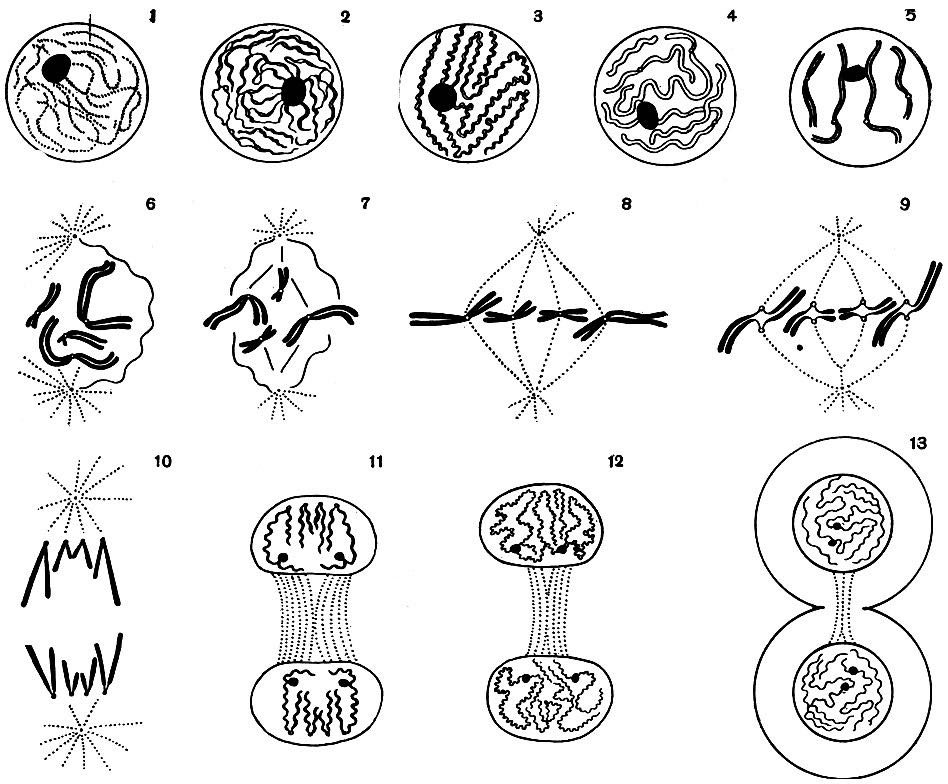
\includegraphics[scale=0.3]{meiosis}
\end{center}


\newpage
\vspace{0.2in}

\makebox[\textwidth]{Команда:\enspace\hrulefill}

\begin{center}
ЭРА III
\end{center}

\begin{questions}


\question Имеется 2 стандартные игральные кости с 6 гранями. Васе для победы нужно выкинуть в сумме 4 и больше. Какова вероятность, что Вася выиграет?

\begin{solution}
$1-3/36=11/12$
\end{solution}

\question Найдите $\E(\text{Ъ})$, если космическая функция плотности $f_\text{Ъ}(\text{ъ}) = \frac{1}{2}e^{-|\text{ъ}|}$, $\text{ъ} \in R$.

\begin{solution}
0
\end{solution}

\question Известно, что $P(A) = P(B) = 1$. Найдите $P(A\Delta B)$
\footnote{$A\Delta B = (A \cap \bar B) \cup ( \bar A \cap B)$}.

\begin{solution}
0
\end{solution}

\question К остановке автобусы подходят строго по расписанию. Является ли это пуассоновским потоком?

\begin{solution}
Нет, это не случайная величина.
\end{solution}

\question Известно что $\P(A) = 1$, $\P(B)=1$. Верно ли, что события А и B независимы?

\begin{solution}
 да
\end{solution}

\question Маша и Ваня играют в игру: ставят на бумаге точку наугад на отрезке от 0 до 100. Маша уже сделала свой ход. Оказалось, что она выбрала точку 40. Найдите вероятность того, что после хода Вани сумма их точек не будет превышать 60.

\begin{solution}
 0.2
\end{solution}

\question Маша, Ваня и Петя играют в игру: ставят на бумаге точку наугад в любом месте на отрезке от 0 до 100. Маша сделала ход, поставила точку. Оказалось, что она выбрала число 40. Найдите вероятность того, что после ходов Вани и Пети, сумма их чисел будет не более 60.

\begin{solution}
 0.02
\end{solution}

\question Найдите вероятность того, что величина $X$ попадёт на отрезок $[0;4]$, если она равномерно распределена на отрезке $[2;18]$.

\begin{solution}
 $2/16=1/8=0.125$
\end{solution}

\question Допустим, в результате галактической переписи обнаружено, что темноволосые матери с темноволосыми дочерьми составили 0.06 обследованных семей, темноволосые матери и светловолосые дочери --- 0.1, светловолосые матери и темноволосые дочери --- 0.14, а светловолосые матери и светловолосые дочери --- 0.7. Найдите условную вероятность того, что дочь имеет темные волосы, если мать темноволосая.

\begin{solution}
 $0.06/(0.06+0.1)=0.375$
\end{solution}


\end{questions}

\end{document}
